\begin{tikzpicture}
	\begin{axis}[
		title={Gaussian Pulse as a CT Signal},
		xlabel={$t$},
		ylabel={$g(t)$},
		xmin=-5, xmax=5,
		ymin=0, ymax=1.1,
		grid=major,
		width=12cm,
		height=8cm,
		]
		\addplot[
		color=red,
		thick,
		domain=-5:5,
		samples=200,
		]
		{exp(-x^2 / 2)};
		\node[anchor=west, fill=white, inner sep=2pt] at (axis cs:-4.8,0.9) 
		{$g(t) = e^{-\tfrac{t^2}{2}}$};
	\end{axis}
\end{tikzpicture}
